\documentclass{beamer}
%%%%%%%%%%%%%%%%%%%
% Now set the style TODO: change this!!
%%%%%%%%%%%%%%%%%%%
\usetheme{Madrid}
\usecolortheme{dolphin}
\setbeamertemplate{page number in head/foot}{}
% Get rid of navigation symbols
\setbeamertemplate{navigation symbols}{}
%%%%%%%%%%%%%%%%%
% custom headline
%%%%%%%%%%%%%%%%%
\setbeamertemplate{headline}{%
\leavevmode%
  \hbox{%
    \begin{beamercolorbox}[wd=0.5\paperwidth,ht=2.5ex,dp=1.125ex]{palette tertiary}%
    \hskip0pt plus1filll \insertsubsection \hspace{2pt}
    \end{beamercolorbox}%
    \begin{beamercolorbox}[wd=0.5\paperwidth,ht=2.5ex,dp=1.125ex]{palette secondary}%
    \hskip 2pt \insertsection
    \end{beamercolorbox}%
  }
}
%%%%%%%%%%
% Packages
%%%%%%%%%%
\usepackage[utf8]{inputenc}
\usepackage{booktabs}
\usepackage{caption}
\usepackage{amssymb}
\usepackage{pifont}

\DeclareCaptionFormat{smol}{ \tiny {\color{blue}Fig#2} #3}

%%%%%%%%%%
% metadata
%%%%%%%%%%
\author[NNPDF]{
Christopher Schwan and
Rosalyn Pearson and
Felix Hekhorn and
Tommaso Giani and
Juan Cruz-Martinez and
Roy Stegeman and
Michael Wilson and
Zahari Kassabov and
Tanjona Rabemananjara
}
\date{PDF4LHC}
\AtBeginSection[]{
   \begin{frame}
   \vfill
   \centering
   \begin{beamercolorbox}[sep=8pt,center,shadow=true,rounded=true]{title}
     \usebeamerfont{title}\insertsectionhead\par
   \end{beamercolorbox}
   \vfill
   \end{frame}
}

\begin{document}
% for footer
\title{NNPDF}
\section{Theory Developments}
\author[Rosalyn Pearson]{}
\institute{University of Edinburgh}
\subsection{Nuclear and deuteron uncertainties}


\begin{frame}[fragile]{Deuteron and nuclear uncertainties}
We use an {\bf uncertainty} rather than a correcting the central value.
\newline
Theory covariance formalism previously developed in NNPDF.
      \begin{block}{Theory covariance matrix \tiny{ \textcolor{green}{[Ball, Nocera, Pearson: Eur.Phys.J.C 79 (2019) 3, 282 \& Eur.Phys.J.C 81 (2021) 1, 37]}}}
        \begin{equation}
            S_{ij} = \frac{1}{N_{rep}} \sum_k^{N_{rep}} \Delta_i^{(k)}\Delta_j^{(k)}
        \end{equation}
        \begin{equation}
            \Delta_i^{(k)} = T_i^{N}[f_{N}^{(k)}] - T_i^{N}[f_{p}]
        \end{equation}
      \end{block}
      
    \textbf{Deuteron:} NNLO deuteron PDFs fitted in NNPDF methodology 
    
    \textbf{Heavy nuclear:} NLO heavy nuclear PDFs from nNNPDF2.0 \tiny{ \textcolor{green}{[Abdul Khalek et al.: JHEP 09 (2020) 183]}}
  \begin{table}
    \caption{$\chi^2$ per deuteron/nuclear dataset}
        \resizebox{\linewidth}{!}{
    \begin{tabular}{rllllllll}
      \toprule
      Fit & {\bf Total} & BCDMS d & SLAC d & NMC p/d & E866/NuSea p/d & E605 Cu & NuTeV Fe & CHORUS Pb \\
      \midrule
      NNPDF4.0 & {\bf 1.174} & 1.015 & 0.4972 & 0.8194 & 0.3971 & 0.4907 & 0.4602 & 0.9372 \\
      No nuc unc & {\bf 1.265} & 1.313 & 0.8217 & 0.8167 & 0.8195 & 1.154 & 0.4569 & 1.165 \\
      \bottomrule
    \end{tabular}}
  \end{table}
\end{frame}

\begin{frame}{Per-point uncertainties}
\footnotesize{Deuteron (top) and heavy nuclear (bottom) }
\newline
\footnotesize{\textcolor{violet}{{\bf C:} experimental uncertainties}}
\newline
\footnotesize{\textcolor{orange}{{\bf S:} theory uncertainties (nuclear)}}
\newline
\footnotesize{\textcolor{cyan}{{\bf C+S:} total}}
  \begin{figure}
    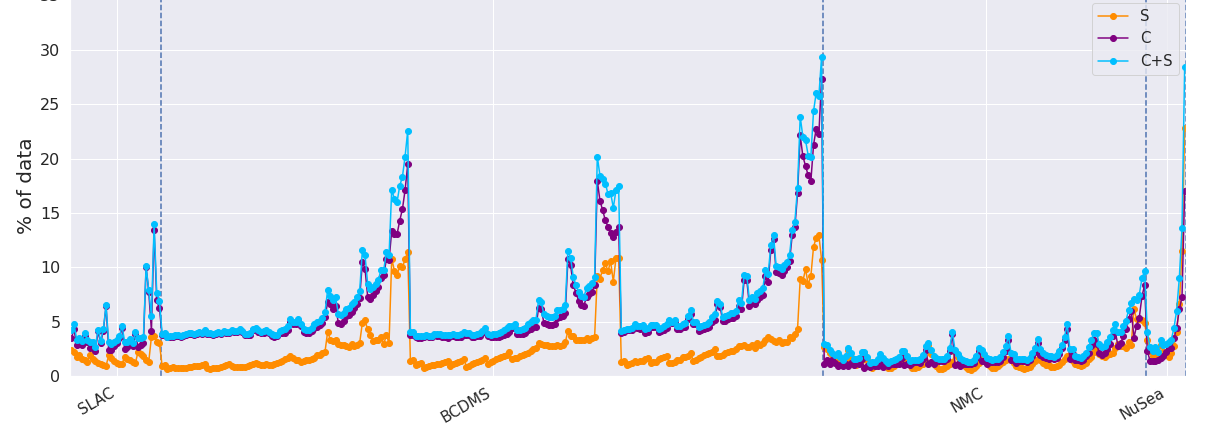
\includegraphics[width=85mm]{nuclear_uncs/diagdeut.png}
    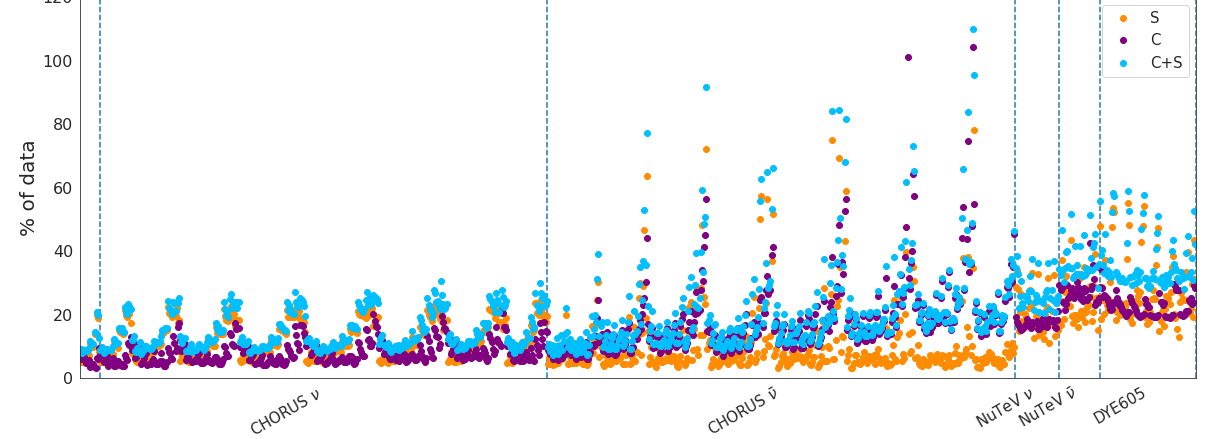
\includegraphics[width=85mm]{nuclear_uncs/diagnuc.png}
  \end{figure}
\end{frame}


\section{PDF properties and their implementation}

\section{The new NNPDF4.0 methodology: \texttt{n3fit}}
\definecolor{darkgreen}{rgb}{0.0, 0.5, 0.13}
\newcommand{\gct}{\color{darkgreen}\checkmark}
\newcommand{\rma}{\color{red}\ding{55}}
\newcommand{\bct}{\color{blue}\checkmark}

\author[Juan Cruz-Martinez]{}
\institute{University of Milan}

\subsection{Hyperoptimization and K-folding}

\begin{frame}{Beyond the PDF fit: fitting the methodology}

    The main objective of NNPDF is to minimize choices that can bias the PDF:

    \begin{columns}
        \column{0.7\linewidth}
        \begin{itemize}
            \item[\rma] Functional form $\longrightarrow$ Neural Networks
            \item[\rma] However: NN are defined by set of parameters!
        \end{itemize}

        \vspace{0.2cm}

        Humans are good at recognising patterns but selecting the best
        set of parameters is a slow process and systematic success is not guaranteed
        \column{0.2\linewidth}
        
\includegraphics[width=\textwidth]{juan_future_hyperopt/kasparov.jpg}

        
\includegraphics[width=\textwidth]{juan_future_hyperopt/alphazero.jpg}
        \column{0.1\linewidth}
    \end{columns}

    \vspace{0.2cm}

    To overcome this selection problem we implement a {\color{blue}  hyperparameter scan}: let the computer decide automatically

    \begin{itemize}
        \item[\gct] Scan over thousands of hyperparameter combinations
        \item[\gct] Define a reward function to grade the model
        \item[\gct] Check the generalization power of the model
    \end{itemize}

\end{frame}

\begin{frame}
    \frametitle{Hyperparameter scan} 
    Each blue dot corresponds to a fit of a different set of hyperparameters:
    { 
        \centering 

        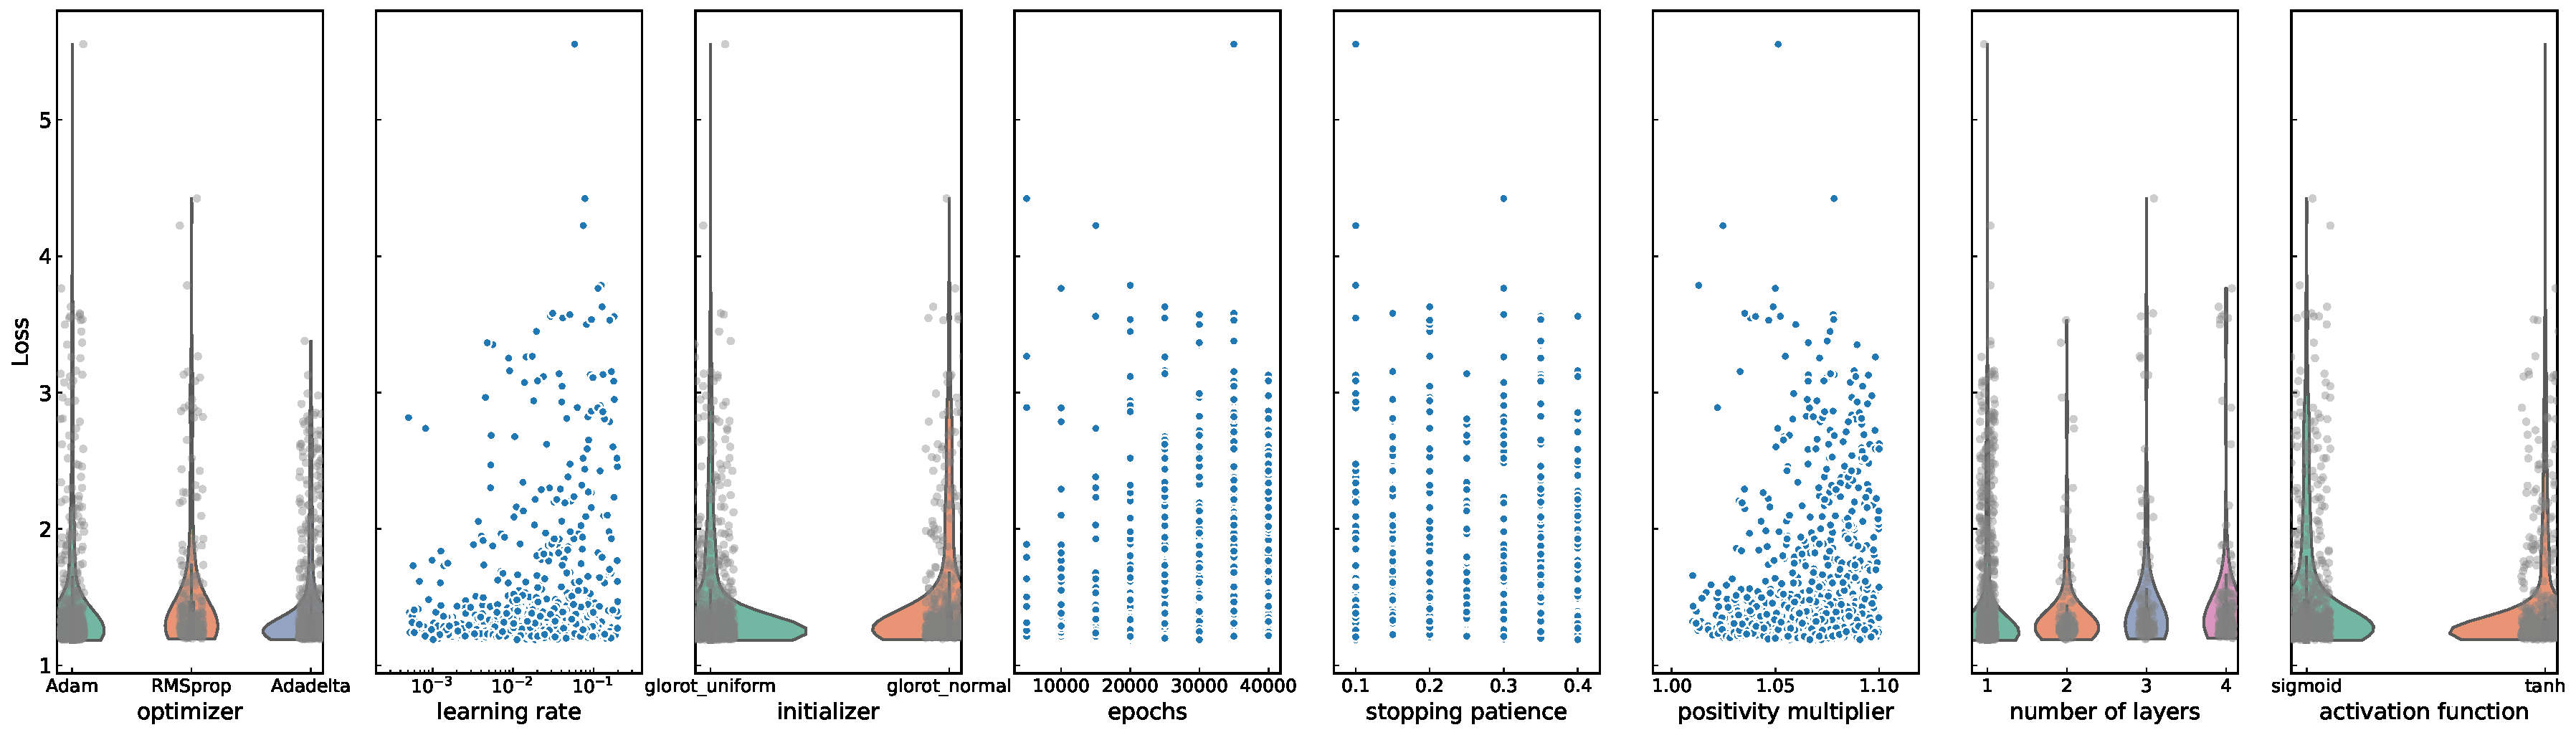
\includegraphics[width=\textwidth]{juan_future_hyperopt/dis-fullpage.pdf}
        Thousands of fits for the hyperoptimization algorithm to choose:

        \begin{columns} \small
            \column{0.35\paperwidth}
            \begin{itemize}
                \item[\bct] Optimizer
                \item[\bct] Initializer
                \item[\bct] Stopping Patience
                \item[\bct] Number of Layers
            \end{itemize}
            \column{0.35\paperwidth}
            \begin{itemize}
                \item[\bct] Learning Rate
                \item[\bct] Epochs
                \item[\bct] Positivity Multiplier
                \item[\bct] Activation Function
            \end{itemize}
        \end{columns}
    } \vfill
\end{frame}

\begin{frame}
    \frametitle{Hyperoptimization: reward and generalization}
    If we use as hyperoptimization target the $\chi^{2}$ of the fitted data, we risk finding the hyperparameter set that
    better overfits.


    \vfill

    \begin{columns}
        \column{0.75\linewidth}
        We avoid this problem by adopting \textbf{$\boldsymbol{k}$-folding}:

        \begin{itemize}
            \item Divide the data into $k$ sets.
            \item Leave one set out and fit the $k-1$ sets left.
            \item Optimize the average $\chi^{2}$ of the $k$ non-fitted sets.
        \end{itemize}
        \column{0.25\linewidth}
        
\includegraphics[width=\textwidth]{juan_future_hyperopt/doctor.jpg}
    \end{columns}

    \vspace{0.4cm}

    Example of function to hyperoptimize:

    \begin{equation*}
        \text{Loss}(optimizer\_name,\ depth\_of\_network) = \frac{1}{k}\displaystyle\sum^{i}_{k} \frac{\chi^{2}_{i}}{N_{i}}
    \end{equation*}

    Where we are computing the $\chi^{2}$ for the data that did not enter the fit. This ensures that the methodology
    can accommodate well even data that has never been seen by the fit.

\end{frame}


\section{Validating the Methodology}
\newcommand{\shift}{\eta}
\newcommand{\vv}[1]{\boldsymbol{#1}}
\newcommand{\erep}{\mathbf{E}_{\epsilon}}
\newcommand{\eshift}{\mathbf{E}_{\shift}}
\newcommand{\ndata}{N_{\rm data}}
\newcommand\Fontvi{\fontsize{8}{7.2}\selectfont}

\makeatletter
\newcommand{\leqnomode}{\tagsleft@true\let\veqno\@@leqno}
\newcommand{\reqnomode}{\tagsleft@false\let\veqno\@@eqno}
\makeatother

\title{NNPDF}
\author[Michael Wilson]{Christopher Schwann and Rosalyn Pearson and Michael Wilson}
\institute{University of Edinburgh}
\date{PDF4LHC}

\subsection{Closure testing NNPDF4.0}
\begin{frame}
    \frametitle{Closure Test}
    \Fontvi
    \begin{columns}[t]
    \column{0.5\textwidth}
    Fit replicas to pseudodata in usual way
    \leqnomode
    \begin{equation}\label{eq:dataassum}
    \begin{split}
        \vv{y} &= \vv{f} + \vv{\shift} + \vv{\epsilon} \\
        &= \vv{z} + \vv{\epsilon},
    \end{split}
    \end{equation}
    where $\vv{\shift} \sim \mathcal{N}(0, C)$ and $\vv{\epsilon} \sim \mathcal{N}(0, C)$ are sampled independently.
    
    Use predictions from an input PDF as proxy for $\vv{f}$.

    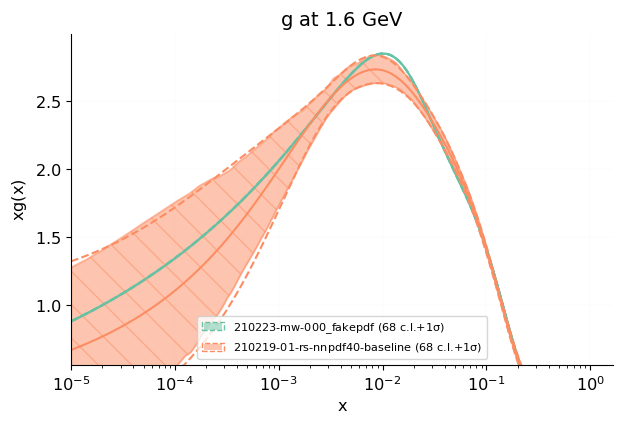
\includegraphics[scale=0.3]{closure_test/plot_pdfs_g.png}
    
    Sampling a random NNPDF replica as the input PDF for a closure test.
    \column{0.5\textwidth}
    \reqnomode
    Allows testing of methodology, if the input assumptions hold.

    \vspace{8pt}
    For example:
    \vspace{8pt}
    
    \textbf{Bias}: difference between central prediction and true observable

    \vspace{8pt}
    \textbf{Variance}: uncertainty of replica predictions

    \vspace{8pt}
    
    Bias is a stochastic variable. If PDF uncertainty is faithful then
    \begin{equation}
        \eshift[{\rm bias}] = {\rm variance}
    \end{equation}

    \vspace{8pt}
    
    High demand on resources - made feasible with \texttt{n3fit}
    \end{columns}
\end{frame}
%
\begin{frame}\frametitle{Preliminary results}
    \Fontvi
    Compare first moments:

    \begin{center}
    \begin{tabular}{lr}
        \toprule
        {} &  $\sqrt{\eshift[{\rm bias}] / \eshift[{\rm variance}]}$\\
        \midrule
        Total      & 1.11 $\pm$ 0.5 \\
        \bottomrule
        \end{tabular}
    \end{center}

    \vspace{8pt}
    Alternatively look at the respective distributions

    \vspace{8pt}
    \begin{center}
        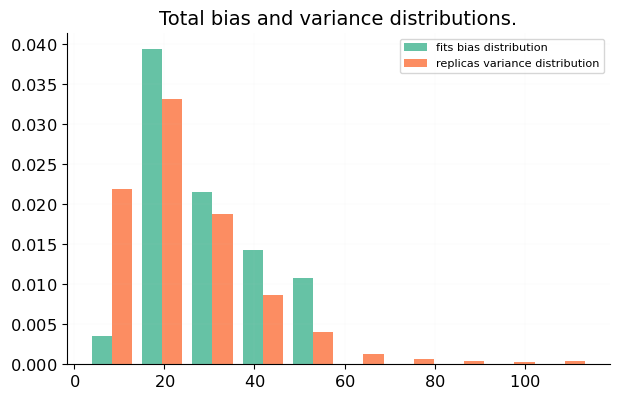
\includegraphics[scale=0.3]{closure_test/plot_bias_variance_distributions_3.png}
    \end{center}

    \vspace{8pt}
    Bias distribution sampled with 25 fits, 40 replicas each.

\end{frame}
\newcommand{\hlme}[1]{{\color{red}\bf #1}}

\author[Juan Cruz-Martinez]{}
\institute{University of Milan}

\subsection{Back to the future}

\begin{frame}{How can we future-proof the methodology?}{Do we trust our errorbands?}

    \small
    The smaller error bands in the NNPDF4.0 fits are driven both by the increased amount of data and the
    improved methodology.
    But there are still kin. regions not covered by data!

    \begin{columns}
        \column{0.6\linewidth}
        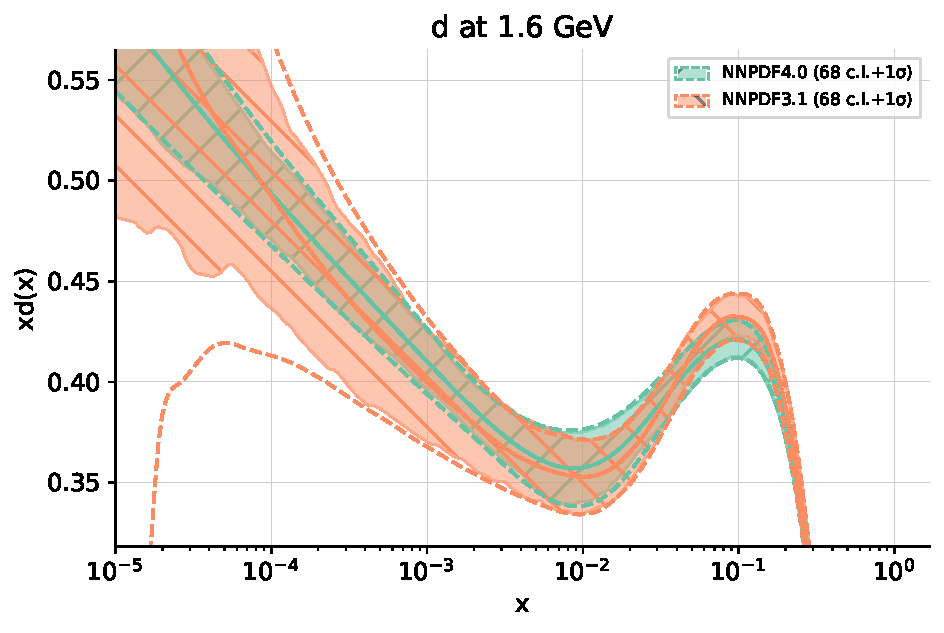
\includegraphics[width=1.0\textwidth]{juan_future_hyperopt/dquark.pdf}

        \column{0.4\linewidth} \vspace{-2.3cm} {

            Ideally: design an experiment for the regions not covered by fitted-data!

            \vspace{0.3cm}

            Problem: we want the results before 2050...

        }
    \end{columns}

    \vspace{-0.3cm}

    \begin{columns}
        \column{0.7\linewidth}
        Solution: chronologically ordered subsets of data to test unseen regions, we named this ``future tests``.

        \column{0.3\linewidth}
        \vspace{-1.9cm}
        \begin{figure}
            \captionsetup{format=smol}
            
\includegraphics[width=0.7\textwidth]{juan_future_hyperopt/tardisdelorean.jpg}
            \caption{\tiny Other valid and certified future-testing methods}
        \end{figure}
    \end{columns}



\end{frame}


\begin{frame}{Future tests}{for more information see \href{https://arxiv.org/pdf/2103.08606.pdf}{\color{blue} arxiv:2103.08606}}

    \begin{columns}
        \column{0.60\linewidth}
        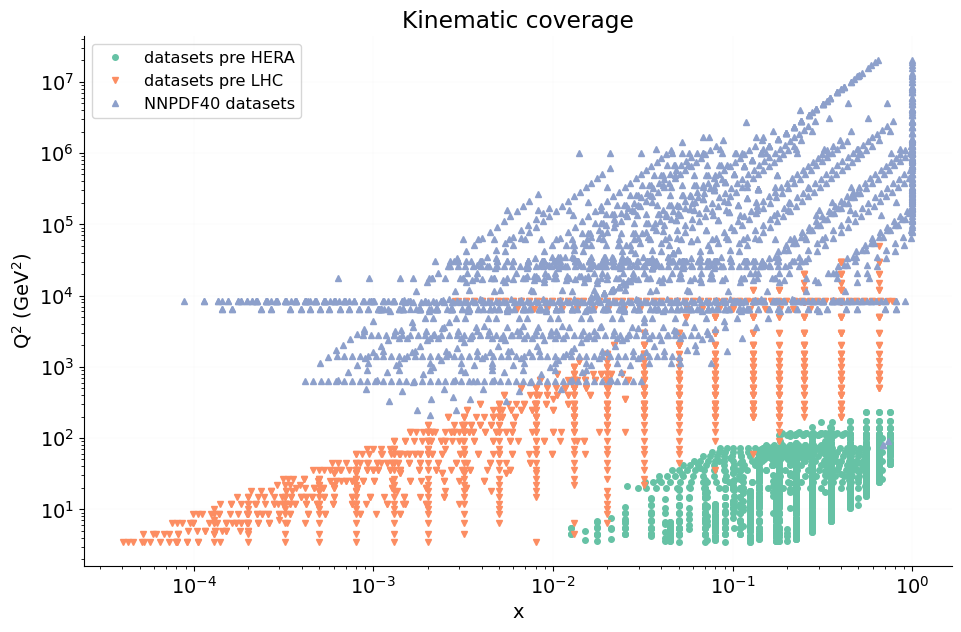
\includegraphics[width=\textwidth, height=0.8\textheight]{juan_future_hyperopt/kincov.png}
        \column{0.46\linewidth}
        \vspace{-0.9cm}
        \only<1>{
            \begin{table}
                \tiny
                \centering
                \caption*{\scriptsize $\chi^{2}/N$ (only exp. covmat)}
                \begin{tabular}{c | c c c} \toprule
                    (dataset) & NNPDF4.0 & pre-LHC & pre-Hera  \\ \midrule
                    pre-HERA  & 1.09 & 1.01 & 0.90 \\
                    pre-LHC   & 1.21 & 1.20 & \hlme{23.1} \\
                    NNPDF4.0  & 1.29 & \hlme{3.30} & \hlme{23.1} \\
                    \bottomrule
                \end{tabular}
            \end{table}
        }
        \only<2>{
            \begin{table}
                \tiny
                \centering
                \caption*{\scriptsize $\chi^{2}/N$ (exp. and PDF covmat)}
                \begin{tabular}{c | c c c} \toprule
                    (dataset) & NNPDF4.0 & pre-LHC & pre-Hera  \\ \midrule
                    pre-HERA  &  & & 0.86 \\
                    pre-LHC   &  & 1.17 & \hlme{1.22} \\
                    NNPDF4.0  & 1.12 & \hlme{1.30} & \hlme{1.38} \\
                    \bottomrule
                \end{tabular}
            \end{table}
        }


        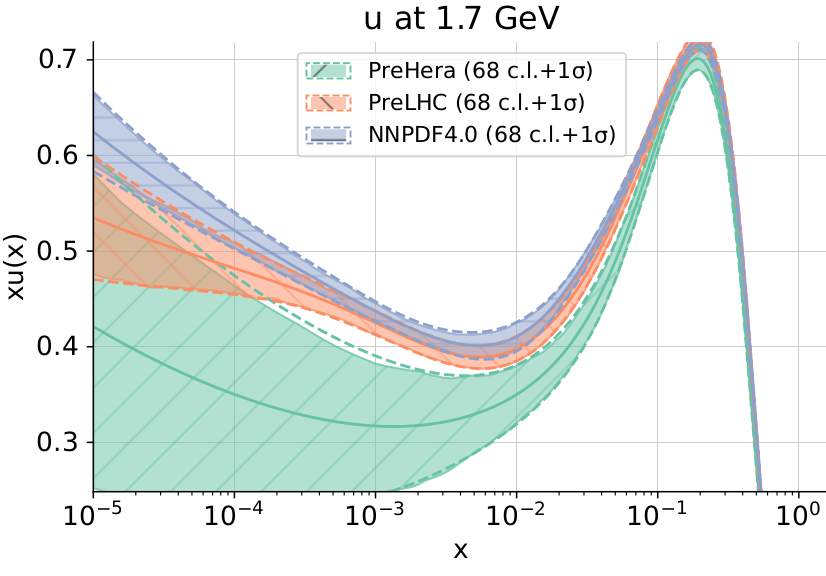
\includegraphics[width=1.0\textwidth]{juan_future_hyperopt/diffu}

    \end{columns}
\end{frame}


\section{Dataset selection}

\section{PDF delivery}

\section{Additional slides}
\title{NNPDF}
\author[Rosalyn Pearson]{}
\institute{University of Edinburgh}
\date{PDF4LHC}

\begin{frame}{Extra: Nuclear and deuteron observables}
\footnotesize{Deuteron (top) and heavy nuclear (bottom) }
  \begin{figure}
    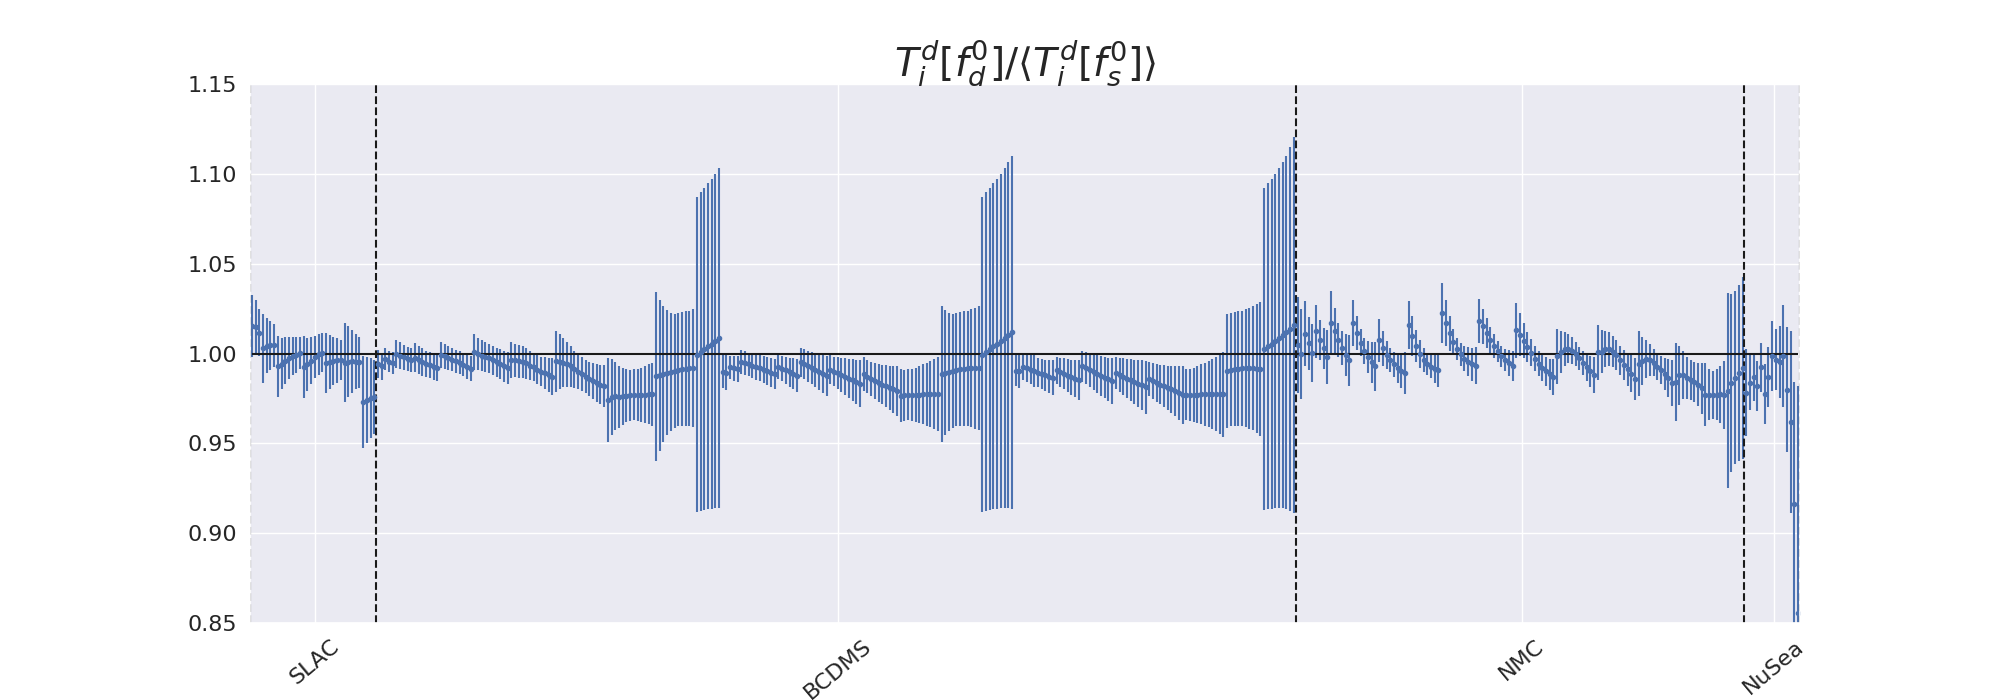
\includegraphics[width=90mm, trim={30mm, 0, 30mm, 0}]{nuclear_uncs/obsdeut.png}
    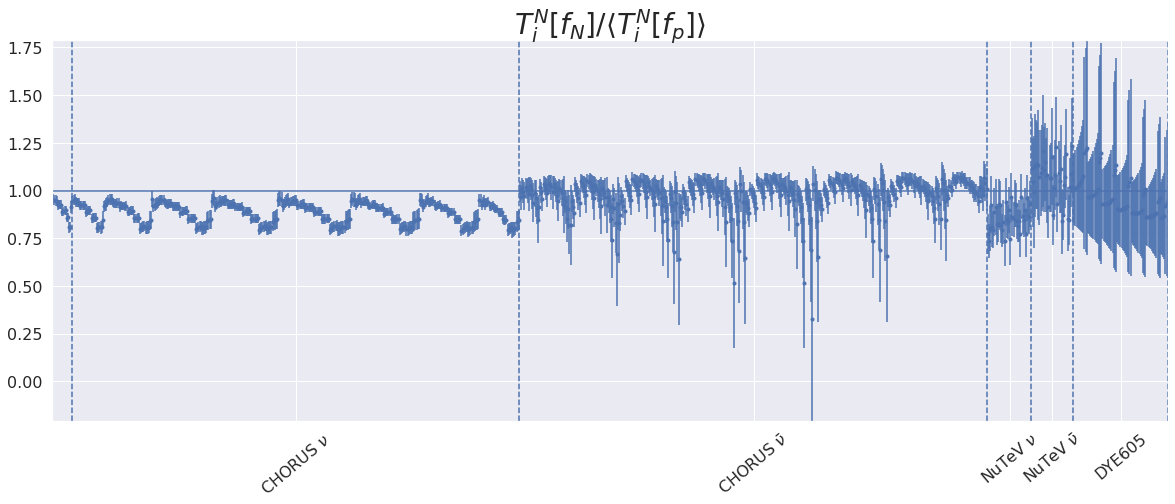
\includegraphics[width=85mm]{nuclear_uncs/obsnuc.png}
  \end{figure}
\end{frame}

\begin{frame}{Extra: deuteron uncertainties}

\begin{block}{Deuteron data}
{\bf Deuteron only} $F_2^d$: SLAC, BCDMS  $\to T_i^d[f_d]$
\newline
{\bf Mixed} $F_2^d/F_2^p$ \& $\sigma_{pd}^{DY}/\sigma_{pp}^{DY}$: NMC, DYE866/NuSea  $ \to T_i^d[f_d, f_p]$
\end{block}
Standard is to use isoscalar PDFs in place of deuteron: $f_s \equiv \frac{1}{2}(f_p + f_d)$
Now 
\begin{equation}
\Delta_i^{(k)} = \begin{cases}
T_i^d[f_d^{(k)}] - T_i^d[f_s^{(0)}] & i \in \text{deuteron only}\\
T_i^d[f_d^{(k)}, f_p^{(0)}] - T_i^d[f_s^{(0)}, f_p^{(0)}] & i \in \text{mixed}
\end{cases}
\end{equation}
\end{frame}

\begin{frame}{Extra: heavy nuclear uncertainties}

\begin{block}{Heavy nuclear data $T_i^N[f_N]$}
{\bf Cu}: DYE605,  $N=64$
\newline
{\bf Fe}: NuTeV (\& EMC), $N=56$
\newline
{\bf Pb}: CHORUS, $N=208$
\end{block}
\begin{equation}
\Delta_i^{(k)} = T_i^{N}[f_{N}^{(k)}] - T_i^{N}[f_{p}]
\end{equation}
Where 
\begin{equation}
\begin{split}
    T_i^N[f_N] = \frac{1}{A} (ZT_i[f_{p/N} + (A-Z)T_i[f_{n/N}] \\
    T_i^N[f_p] = \frac{1}{A} (ZT_i[f_p] +  (A-Z)T_i[f_n]
\end{split}
\end{equation}
\end{frame}
\begin{frame}{Extra: Correlation matrix}
  \begin{figure}
  \centering
    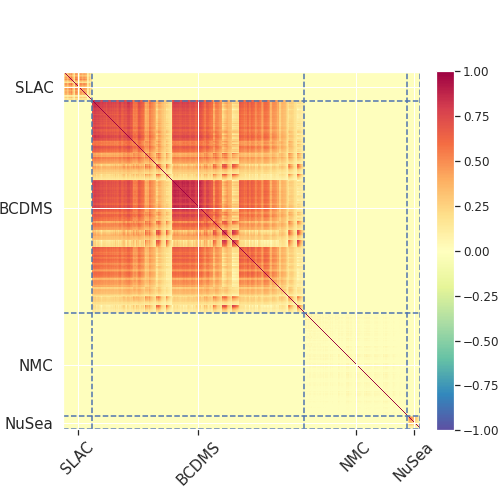
\includegraphics[width=40mm]{nuclear_uncs/covexpdeut.png}
    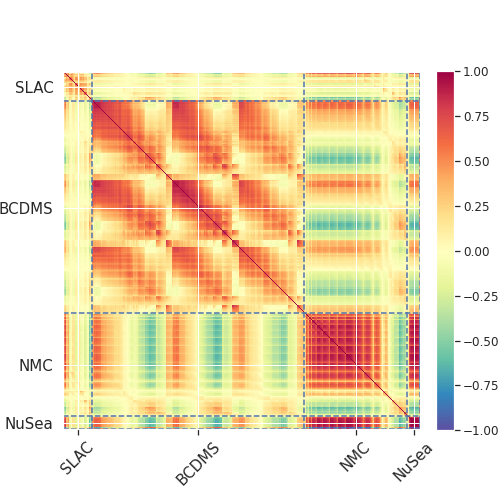
\includegraphics[width=40mm]{nuclear_uncs/covtotdeut.png}
    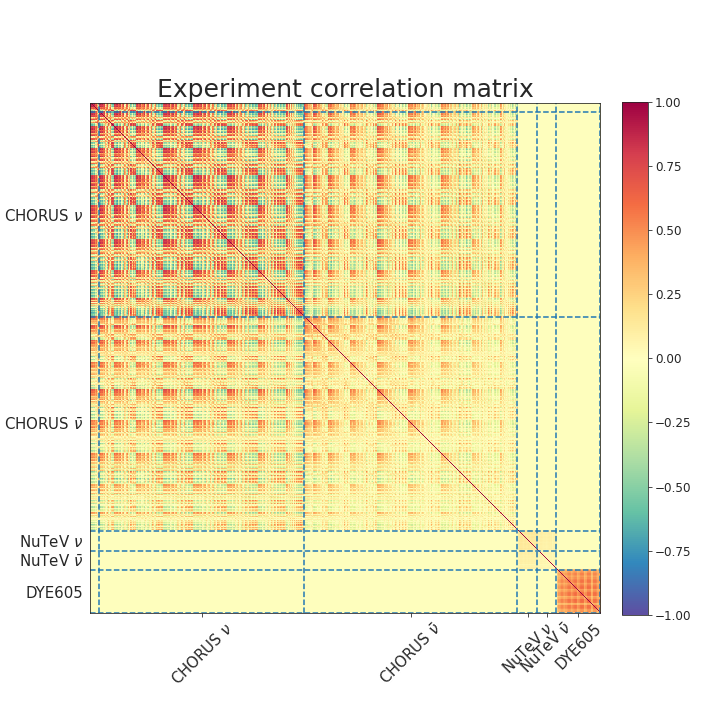
\includegraphics[width=40mm]{nuclear_uncs/covexpnuc.png}
    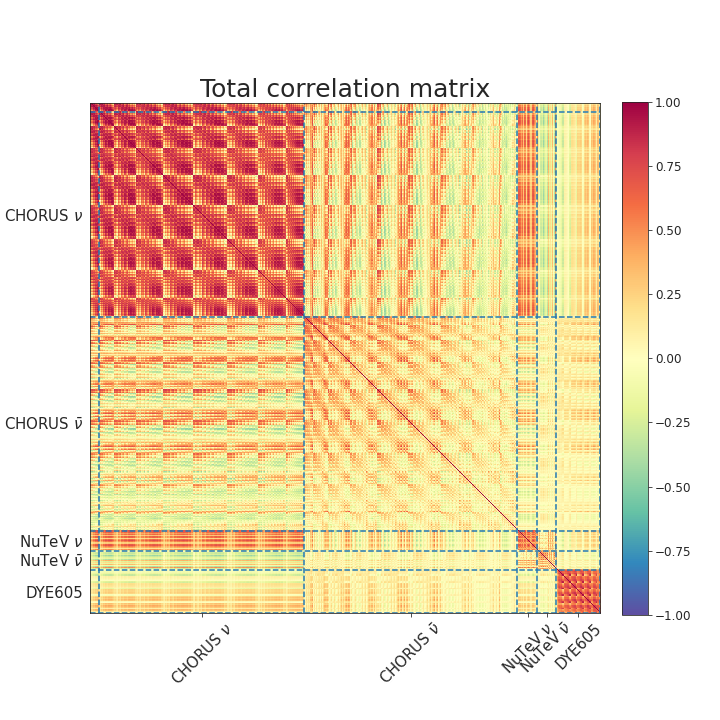
\includegraphics[width=40mm]{nuclear_uncs/covtotnuc.png}
  \end{figure}
  \end{frame}
\begin{frame}{Extra: Nuclear correction}
\begin{itemize}
\item Can also ``shift" the observables $T_i^{(N/d)}[f_(p/s)^{(0)}] \to T_i^{(N/d)}[f_{(N/d)}^{(0)}]$
\item Uncertainty is correspondingly reduced
\end{itemize}
  \begin{figure}
    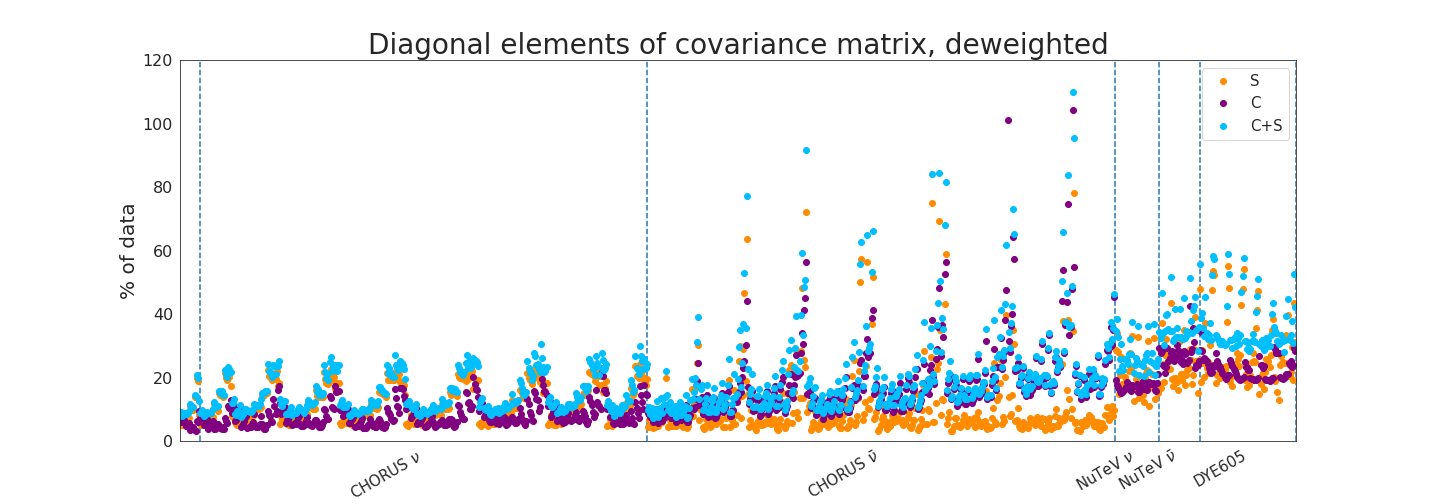
\includegraphics[width=85mm]{nuclear_uncs/diagnuc_title.png}
    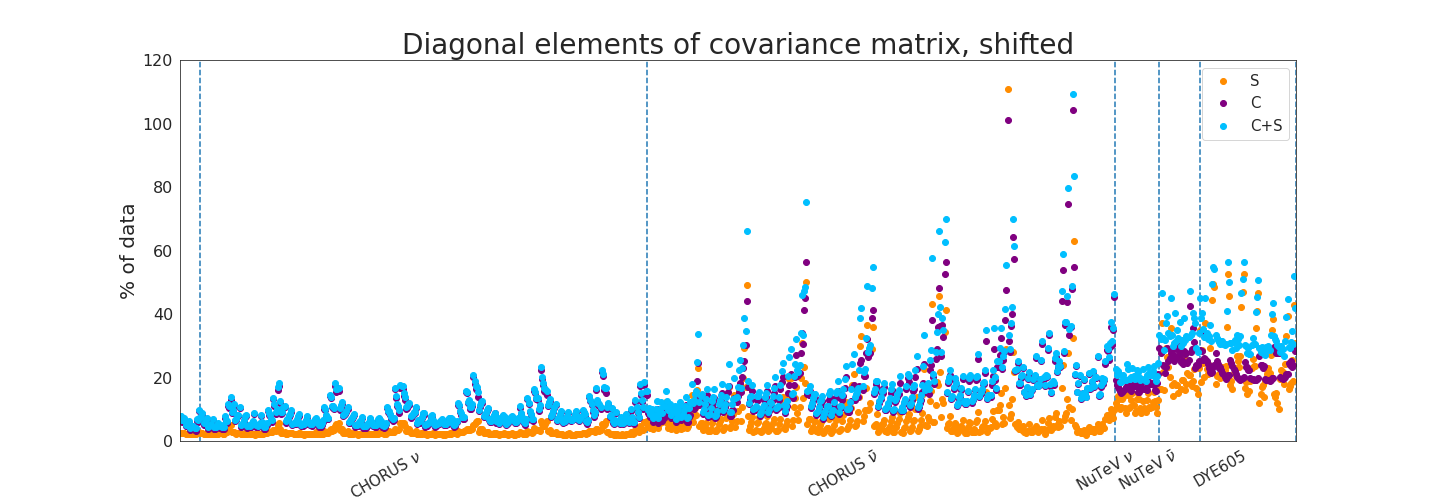
\includegraphics[width=85mm]{nuclear_uncs/diagnucshift.png}
  \end{figure}
\end{frame}
\begin{frame}{Extra: Deuteron correction}
Comparing deuteron correction to MMHT \tiny{ \textcolor{green}{[Harland-Lang et al.: Eur. Phys. J. C 75(5), 204 (2015)]}}
  \begin{figure}
    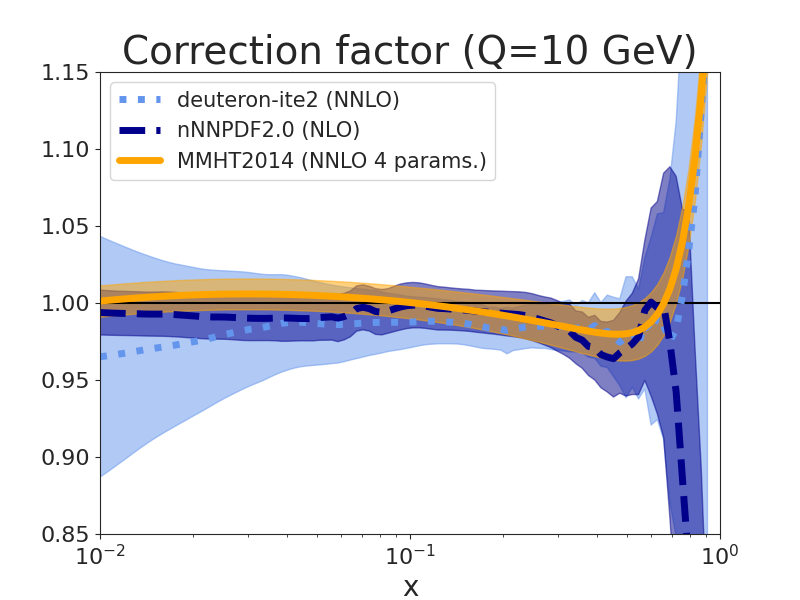
\includegraphics[width=90mm]{nuclear_uncs/corrfactor.png}
  \end{figure}
\end{frame}


\end{document}
